\section{Related Works}
Several efficient algorithms have been proposed for
FIM. Some of the most famous are Apriori\cite{apriori}, FP-Growth\cite{fp_growth},...
All of these algorithms have the same input and the same output. However, the difference is
the strategies and data structures that these algorithms employ to discover frequent itemsets
efficiently. More specifically, FIM algorithms differ in whether they use a depth-first or
breadth-first search, the type of database representation that they use internally or
externally, how they generate or determine the next itemsets to be explored in the search
space, and how they count the support of itemsets to determine if they satisfy the
minimum support constraint.

\subsection{Breadth-first search and depth-first search}
First of all, we can use the letters $a, b, c,...$ to represent items in Table \ref{tab:example_dataset_in_real}.
Where $apple$ is represented by $a$, $banana$ is represented by $b$, $cherry$ is represented by $c$ and $mango$ is represented by $d$.
Then, we can represent it:
\begin{table}[H]
    \centering
    \caption{Example of a dataset of transactions}
    \label{tab:example_dataset_in_real_encode}
    \begin{tabular}{|c|l|}
        \hline
        \textbf{Tid} & \textbf{Itemsets} \\
        \hline
        1            & a, b, c           \\
        2            & a, d              \\
        3            & a, c              \\
        4            & d, c              \\
        5            & a, d, c           \\
        \hline
    \end{tabular}
\end{table}

Most of the existing itemset mining algorithms can be described as either using a breadth-first
search or a depth-first search. Assume that there are $m$ items in a database. A breadth-
first search algorithm (also called a level-wise algorithm) such as Apriori\cite{apriori} explores the search
space of itemsets by first considering 1-itemsets, then 2-itemsets, 3-itemsets . . . , and lastly
$m$-itemsets.

\begin{figure}
    \caption{Search space of all possible itemsets for the running example}
    \label{fig:search_space}
    \centering
    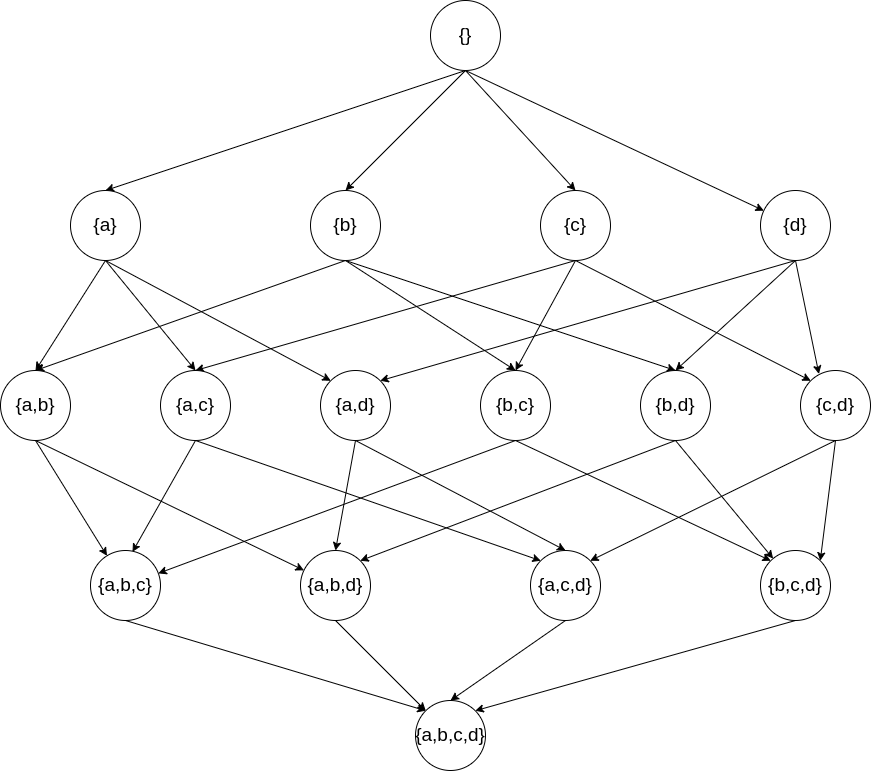
\includegraphics[width=0.9\textwidth]{chapter1/image/space.png}
\end{figure}

For example, Figure \ref{fig:search_space} depicts the search space of all possible itemsets for the
running example. In this figure, the search space is represented as
a Hasse diagram\footnote{A Hasse diagram draws an arrow from an itemset $X$ to another itemset $Y$ if and only if $X \subseteq Y$ and $|X| + 1 = Y$.}
A breadth-first search algorithm will first consider 1-itemsets \{$a$\}, \{$b$\}, \{$c$\}, \{$d$\}. Then,
it will generate 2-itemsets such as \{$a, b$\}, \{$a, c$\}, \{$a, d$\}, and then 3-itemsets, and so on, until it
generates the itemset \{$a, b, c, d$\} containing all items. On the other hand, depth-first search
algorithms such as FPGrowth, H-Mine and LCM start from each 1-itemset and then recursively try to append items to the current itemset to generate larger itemsets.
For example, in the running example, a typical depth-first search algorithm would explore itemsets in that
order: \{$a$\}, \{$a, b$\}, \{$a, b, c$\}, \{$a, b, c, d$\}, \{$a, b, d$\},
\{$a, c$\}, \{$a, c, d$\}, \{$a, d$\}, \{$b$\}, \{$b, c$\}, \{$b, c, d$\},
\{$b, d$\}, \{$c$\}, \{$c, d$\}, \{$d$\}.

To design an efficient FIM algorithm, it is important that the algorithm avoid exploring
the whole search space of itemsets because the search space can be very large. To reduce
the search space, search space pruning techniques are used.

\subsection{Apriori: an horizontal breadth-first search algorithm}
Apriori\cite{apriori} is a well-known algorithm for mining frequent itemsets.
It is the first FIM algorithm. Apriori takes a transaction database and the minsup
threshold as input. Apriori uses a standard database representation, as shown in Table
1, also called a horizontal database. The pseudocode of Apriori is given:

\begin{algorithm}
    \caption{Apriori algorithm}
    \begin{algorithmic}[1]
        \State \textbf{Input}: $D$: a horizontal transaction database, $minsup$: a user-specified threshold
        \State \textbf{Output}: the set of frequent itemsets
        \State Scan the database to calculate the support of all items in I;
        \State $F_1 = \{i | i \in I \wedge Supp(\{i\}) \ge minsup\}$; \Comment{Frequent 1-itemsets}
        \State $k = 2$;
        \While{$F_{k} \neq \emptyset$}
        \State $C_k = \{i_1, i_2, ..., i_k | i_1 \in F_1, i_2 \in F_2, ..., i_k \in F_k\}$; \Comment{Generate candidate k-itemsets}
        \State Remove each candidate $X \in C_k$ that contains a $(k-1)$ itemset not in $F_{k-1}$;
        \State Scan the database to calculate the support of each candidate in $C_k$;
        \State $F_k = \{X \in C_k | Supp(X) \ge minsup\}$; \Comment{Frequent k-itemsets}
        \State $k = k + 1$;
        \EndWhile
        \State \textbf{return} $\bigcup_{k=1...k} F_k$;
    \end{algorithmic}
\end{algorithm}

Apriori first scans the database to calculate the support of each item, i.e. 1-itemset.
Then, Apriori uses this information to identify the set of all frequent items, denoted as $F_1$.
Then, Apriori performs a breadth-first search to find larger frequent itemsets.
During the search, Apriori uses the frequent itemsets of a given length $k - 1$
(denoted as $F_{k-1}$) to generate potentially frequent itemsets of length k (denoted as $C_k$). This
is done by combining pairs of items of length k that share all but one item.
For example, if the frequent 1-itemsets are {a}, {b}, {c}, Apriori will combine pairs of
these itemsets to obtain the following candidate 2-itemsets: {a, b}, {a, c} and {b, c}.
After generating candidates of length k, Apriori checks if the $(k - 1)$-subsets of
each candidate are frequent. If a candidate itemset X has an infrequent $(k - 1)$-subset, $X$
cannot be frequent (it would violate the downward-closure property) and it is thus removed
from the set of candidate $k-itemsets$.
Then, Apriori scans the database to calculate the
support of all remaining candidate itemsets in $C_k$. Each candidate having a support
not less than minsup is added to the set $F_k$ of frequent $k-itemsets$. This process
is repeated until no candidates can be generated. The set of all frequent itemsets is then
returned to the user.

Apriori is an important algorithm as it has inspired many other algorithms. However, it
suffers from important limitations. The first one is that because Apriori generates candidates
by combining itemsets without looking at the database, it can generate some patterns that
do not even appear in the database. Thus, it can spend a huge amount of time processing
candidates that do not exist in the database. The second limitation is that Apriori has to
repeatedly scan the database to count the support of candidates, which is very costly.

The third limitation is that the breadth-first search approach can be quite costly in terms of
memory as it requires at any moment to keep in the worst case all $k$ and $k - 1$ itemsets
in memory (for $k > 1$). In terms of complexity, a very detailed complexity analysis of the
Apriori algorithm has been done by Hegland\cite{hegland}. Briefly, the time complexity is $O(m^2n)$,
where $m$ is the number of distinct items and $n$ is the number of transactions.